\section{HÀM SỐ LƯỢNG GIÁC VÀ ĐỒ THỊ}
\subsection{KIẾN THỨC CẦN NHỚ}
\subsubsection{Hàm số $\mathbf{y=\sin x}$}
\vspace{-0.5cm}
	\immini{
	\begin{itemize}
		\item Tập xác định: $\mathscr{D}=\Bbb{R}.$
		\item  Tập giá trị: $ [-1;1]$, tức là \\
		\centerline{$-1\le \sin x\le 1$, $\forall x\in \mathbb{R}.$}
		\item  Hàm số $y=\sin x$ là hàm số lẻ nên đồ thị hàm số nhận gốc tọa độ $O$ làm tâm đối xứng.
	\end{itemize}}{ 
		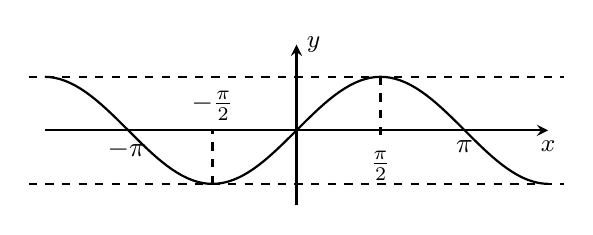
\begin{tikzpicture}[thick,>=stealth,x=1cm,y=1cm,scale=0.68] 
		\draw[->] (-4.7,0) -- (4.7,0) node[below] {\small $x$};
		\draw[->] (0,-1.4) -- (0,1.6) node[right] {\small $y$};
		\draw[thick,samples=100,domain=-4.7:4.7] plot(\x,{sin((\x)*180/pi)});
		\draw (-3.17,0) node[below] {$-\pi$};
		\draw (3.14,0) node[below] {$\pi$};
		\draw[dashed] (-1.57,-1)--(-1.57,0) node[above] {$-\frac{\pi}{2}$};
		\draw[dashed] (1.57,1)--(1.57,-0.2) node[below] {$\frac{\pi}{2}$};
		\draw[dashed] (-5,1)--(5,1);
		\draw[dashed] (-5,-1)--(5,-1);
		\end{tikzpicture}
	}
\begin{itemize}
	\item Hàm số $y=\sin x$ tuần hoàn với chu kì $T=2\pi$, nghĩa là $\sin(x+k2\pi)=\sin x$, với $k \in \mathbb{Z}$.
	\item Hàm số $y=\sin x$ đồng biến trên mỗi khoảng $\left(-\dfrac{\pi}{2}+k 2 \pi ; \dfrac{\pi}{2}+k 2 \pi\right)$, nghịch biến trên mỗi khoảng $\left(\dfrac{\pi}{2}+k 2 \pi ; \dfrac{3 \pi}{2}+k 2 \pi\right)$ với $k \in \mathbb{Z}$.
\end{itemize}
\subsubsection{Hàm số $y=\cos x$}
\vspace{-0.5cm}
\immini{
	\begin{itemize}
		\item Tập xác định: $\mathscr{D}=\Bbb{R}.$
		\item  Tập giá trị: $ [-1;1]$, tức là\\
		\centerline{ $-1\le \cos x\le 1$, $\forall x\in R.$}
		\item  Hàm số $y=\cos x$ là hàm số chẵn nên đồ thị hàm số nhận trục $Oy$ làm trục đối xứng.
	\end{itemize}
	}{
	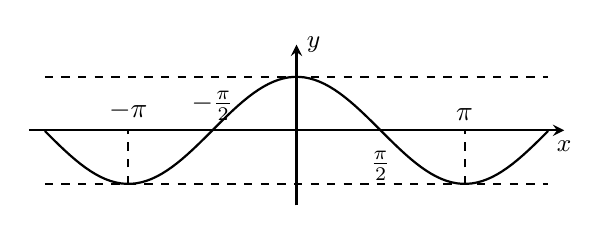
\begin{tikzpicture}[thick,>=stealth,x=1cm,y=1cm,scale=0.68] 
		\draw[->] (-5,0) -- (5,0) node[below] {\small $x$};
		\draw[->] (0,-1.4)-- (0,1.6) node[right] {\small $y$};
		\draw[thick,samples=100,domain=-4.7:4.7] plot(\x,{cos((\x)*180/pi)});
		\draw[dashed] (-3.14,-1)--(-3.14,0) node[above] {$-\pi$};
		\draw[dashed] (3.14,-1)--(3.14,0) node[above] {$\pi$};
		\draw (-1.57,0) node[above] {$-\frac{\pi}{2}$};
		\draw (1.57,-0.2) node[below] {$\frac{\pi}{2}$};
		\draw[dashed] (-4.7,1)--(4.7,1);
		\draw[dashed] (-4.7,-1)--(4.7,-1);
		\end{tikzpicture}}
	\begin{itemize}
		\item Hàm số $y=\cos x$ là hàm số tuần hoàn với chu kì $T=2\pi $, nghĩa là $\cos(x+k2\pi)=\cos x$, với $k \in \mathbb{Z}$.
		\item Hàm số $y=\cos x$ đồng biến trên mỗi khoảng $(-\pi+k 2 \pi ; k 2 \pi)$, nghịch biến trên mỗi khoảng $(k 2 \pi ; \pi+k 2 \pi)$ với $k \in \mathbb{Z}$.
	\end{itemize}
\subsubsection{Hàm số $y=\tan x$}
	\immini{
\begin{itemize}
\item  Điều kiện $\cos x \ne 0 \Leftrightarrow x \ne \dfrac{\pi}{2}+k\pi, k\in \mathbb{Z}$.\\
		Tập xác định: $\mathscr{D}=\mathbb{R}\backslash \left\{\dfrac{\pi}{2}+k\pi, k\in \mathbb{Z}\right\}.$
		\item  Tập giá trị: $\mathbb{R}$; Là hàm số lẻ.
		\item  Là hàm số tuần hoàn với chu kì $T=\pi$, nghĩa là $\tan(x+k\pi)=\tan x$, với $k \in \mathbb{Z}$.
	\end{itemize}
	}{\vspace*{-2\baselineskip}
		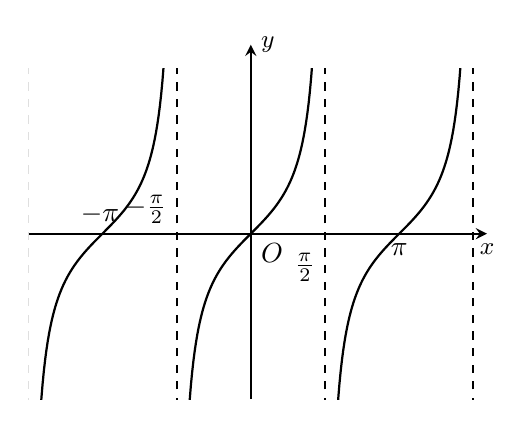
\begin{tikzpicture}[thick,>=stealth,scale=0.6] 
		\draw[->] (-4.7,0) -- (5,0) node[below] {\small $x$};
		\draw[->] (0,-3.5) -- (0,4) node[right] {\small $y$};
		\draw (0,0) node[below right] {$O$};
		\clip(-4.7,-3.5) rectangle (5,3.5);
		\draw[thick,samples=100,domain=-1.325:1.36] plot(\x,{tan((\x)*180/pi)});
		\draw (-3.19,0) node[above] {$-\pi$};
		\draw (3.14,0) node[below] {$\pi$};
		\draw (-1.57,0) node[above left=-0.1] {$-\frac{\pi}{2}$};
		\draw (1.57,-0.2) node[below left=-0.1] {$\frac{\pi}{2}$};
		\draw[dashed] (1.57,-4)--(1.57,5);
		\draw[dashed] (-1.57,-4)--(-1.57,5);
		\draw[dashed] (-4.71,-4)--(-4.71,5);
		\draw[dashed] (4.71,-4)--(4.71,5);
		\draw[thick,samples=100,domain=1.82:4.5] plot(\x,{tan((\x)*180/pi)});
		\draw[thick,samples=100,domain=-4.46:-1.79] plot(\x,{tan((\x)*180/pi)});
		\end{tikzpicture}
	}
\begin{itemize}
	\item Hàm số $y=\tan x$ đồng biến trên mỗi khoảng $\left(-\frac{\pi}{2}+k \pi ; \frac{\pi}{2}+k \pi\right)$ với $k \in \mathbb{Z}$.
\end{itemize}
\subsubsection{Hàm số $y=\cot x$}

\begin{itemize}
\immini{\item  Điều kiện $\sin x \ne 0 \Leftrightarrow x \ne k\pi, k\in \mathbb{Z}$.\\
	Tập xác định: $\mathscr{D}=\mathbb{R}\setminus \left\{k\pi, k\in \mathbb{Z}\right\}.$
	\item  Tập giá trị: $\mathbb{R}.$
	\item  Là hàm số lẻ.
	\item  Là hàm số tuần hoàn với chu kì $T=\pi$, nghĩa là  $\cot(x+k\pi)=\cot x$, với $k \in \mathbb{Z}$.
	\item Hàm số $y=\cot x$ nghịch biến trên mỗi khoảng $(k \pi ; \pi+k \pi)$ với $k \in \mathbb{Z}$.
}{\vspace{-0.6cm}
	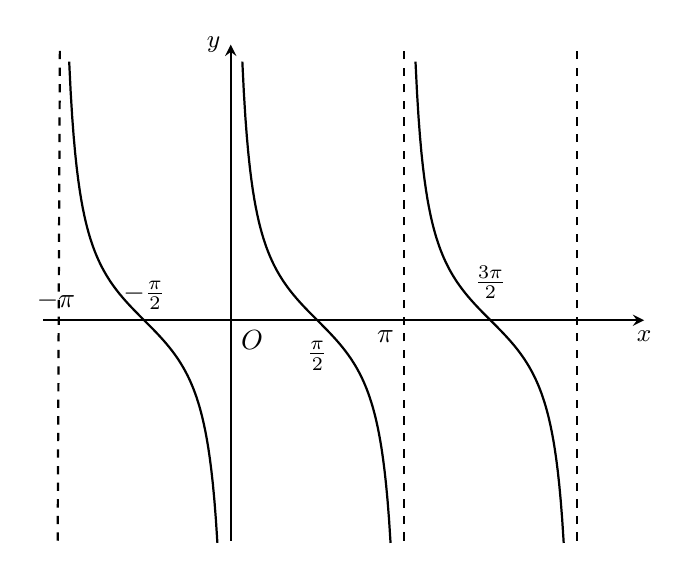
\begin{tikzpicture}[thick,>=stealth,scale=0.7] 
		\draw[->] (-3.4,0) -- (7.5,0) node[below] {\small $x$};
		\draw[->] (0,-4) -- (0,5) node[left] {\small $y$};
		\draw (0,0) node[below right] {$O$};
		\draw[thick,samples=100,domain=0.21:2.9] plot(\x,{cot((\x)*180/pi)});
		\draw[thick,samples=100,domain=0.21:2.9] plot(\x-pi,{cot((\x)*180/pi)});
		\draw[thick,samples=100,domain=0.21:2.9] plot(\x+pi,{cot((\x)*180/pi)});
		%\draw[thick,samples=100,domain=0.21:2.9] plot(\x-2*pi,{cot((\x)*180/pi)});
		\draw (-3.17,0) node[above] {$-\pi$};
		\draw (3.14,0) node[below left=-0.1] {$\pi$};
		\draw (-1.57,0) node[above] {$-\frac{\pi}{2}$};
		\draw (1.57,-0.2) node[below] {$\frac{\pi}{2}$};
		%\draw (-4.71,-0.2) node[below] {$-\frac{3\pi}{2}$};
		\draw (4.71,0.2) node[above] {$\frac{3\pi}{2}$};
		\draw[dashed] (3.14,-4)--(3.14,5);
		\draw[dashed] (-3.14,-4)--(-3.1,5);
		\draw[dashed] (6.28,-4)--(6.28,5);
		%\draw[dashed] (-6.28,-4)--(-6.28,5);
		\end{tikzpicture}}
\end{itemize}

\begin{dang}{Tìm tập xác định của hàm số lượng giác}
	Ta chú ý một số điều kiện sau:
	\begin{enumerate}
		\item $y=\dfrac{f(x)}{g(x)}$ xác định $ \Leftrightarrow g(x)\ne 0$. 
		\item $y=\sqrt[2n]{f(x)}$ xác định $ \Leftrightarrow f(x)\geqslant 0$, trong đó $n\in \mathbb{N}^*$. 
		\item $y=\tan \left[u(x)\right]$ xác định $ \Leftrightarrow u(x)$ xác định và $u(x)\ne \dfrac{\pi}{2}+k\pi,k\in \mathbb{Z}$. 
		\item $y=\cot \left[u(x)\right]$ xác định $ \Leftrightarrow u(x)$ xác định và $u(x)\ne k\pi,k\in \mathbb{Z}$. 
	\end{enumerate}
\end{dang}

\begin{dang}{Tính chẵn lẻ của hàm số}
	Ta thực hiện các bước sau: 
	\begin{enumerate}
		\item[\ding{172}] Tìm tập xác định $\mathscr{D}$ của hàm số -- Tập $\mathscr{D}$ phải đối xứng.
		\item[\ding{173}] Tính $f\left(-x\right)$ (\textit{chỗ nào có biến $x$, ta thay bởi $-x$}) và thu gọn kết quả. Khi đó 
		\begin{itemize}
			\item [$\bullet$] Nếu $f(-x)=f(x)$: hàm số đã cho là hàm chẵn.
			\item [$\bullet$] Nếu $f(-x)=-f(x)$: hàm số đã cho là hàm lẻ.
			\item [$\bullet$] Nếu không rơi vào 2 trường hợp trên, ta kết luận hàm số không chẵn, không lẻ.
		\end{itemize}
	\end{enumerate}
	
	\begin{khung4}{GHI NHỚ}
		\begin{listEX}[2]
			\item [\ding{172}] Hàm số $y=\sin x$ là hàm số lẻ.
			\item [\ding{173}] Hàm số $y=\cos x$ là hàm số chẵn.
			\item [\ding{174}] Hàm số $y=\tan x$ là hàm số lẻ.
			\item [\ding{175}] Hàm số $y=\cot x$ là hàm số lẻ.
		\end{listEX}
	\end{khung4}	
\end{dang}

\begin{dang}{Tìm giá trị lớn nhất - giá trị nhỏ nhất}
	Ta thường dùng một trong 3 phương pháp sau:
	\begin{enumerate}[\faCheckSquareO]
		\item Sử dụng các bất đẳng thức cơ bản
		\begin{listEX}[2]
			\item [\ding{172}] $-1 \leq \sin x \leq 1,\forall x \in \mathbb{R}$;
			\item [\ding{173}] $-1 \leq \cos x \leq 1,\forall x\in \mathbb{R}$;
			\item [\ding{174}] $0 \leq \sin^2x, \cos^2 x\leq 1,\forall x \in \mathbb{R}$;
			\item [\ding{175}]  $0 \leq |\sin x|, |\cos x| \leq 1,\forall x \in \mathbb{R}$.
		\end{listEX}
		\item Sử dụng điều kiện có nghiệm
		\begin{listEX}[1]
			\item [\ding{172}] $\sin x = f(m)$ có nghiệm khi $-1\le f(m) \le 1$.
			\item [\ding{173}] $\cos x = f(m)$ có nghiệm khi $-1\le f(m) \le 1$.
			\item [\ding{174}] $a\sin x + b\cos x = c$ có nghiệm khi $a^2+b^2 \ge c^2$.
		\end{listEX}
		\item Sử dụng bảng biến thiên: Lập bảng biến thiên của hàm số, từ đó, kết luận.
	\end{enumerate}
\end{dang}

